 \documentclass[bachelor, och, labwork]{shiza}
% параметр - тип обучения - одно из значений:
%    spec     - специальность
%    bachelor - бакалавриат (по умолчанию)
%    master   - магистратура
% параметр - форма обучения - одно из значений:
%    och   - очное (по умолчанию)
%    zaoch - заочное
% параметр - тип работы - одно из значений:
%    referat    - реферат
%    coursework - курсовая работа (по умолчанию)
%    diploma    - дипломная работа
%    pract      - отчет по практике
% параметр - включение шрифта
%    times    - включение шрифта Times New Roman (если установлен)
%               по умолчанию выключен
\usepackage{subfigure}
\usepackage{tikz,pgfplots}
\pgfplotsset{compat=1.5}
\usepackage{float}
\usepackage{pdfpages}

\usepackage{titlesec}
\setcounter{secnumdepth}{4}
\titleformat{\paragraph}
{\normalfont\normalsize}{\theparagraph}{1em}{}
\titlespacing*{\paragraph}
{35.5pt}{3.25ex plus 1ex minus .2ex}{1.5ex plus .2ex}

\titleformat{\paragraph}[block]
{\hspace{1.25cm}\normalfont}
{\theparagraph}{1ex}{}
\titlespacing{\paragraph}
{0cm}{2ex plus 1ex minus .2ex}{.4ex plus.2ex}

% --------------------------------------------------------------------------%


\usepackage[T2A]{fontenc}
\usepackage[utf8]{inputenc}
\usepackage{graphicx}
\graphicspath{ {./images/} }
\usepackage{tempora}
\usepackage{kantlipsum}
\usepackage[sort,compress]{cite}
\usepackage{amsmath}
\usepackage{amssymb}
\usepackage{amsthm}
\usepackage{fancyvrb}
\usepackage{listings}
\usepackage{listingsutf8}
\usepackage{longtable}
\usepackage{array}
\usepackage[english,russian]{babel}

%\usepackage[colorlinks=true]{hyperref}
\usepackage{url}

\usepackage{underscore}
\usepackage{setspace}
\usepackage{indentfirst} 
\usepackage{mathtools}
\usepackage{amsfonts}
\usepackage{enumitem}
\usepackage{tikz}

\newcommand{\eqdef}{\stackrel {\rm def}{=}}
\newcommand{\specialcell}[2][c]{%
	\begin{tabular}[#1]{@{}c@{}}#2\end{tabular}}

\renewcommand\theFancyVerbLine{\small\arabic{FancyVerbLine}}

\begin{document}

	\includepdf{yahin-titulnik2.pdf}
	
	%-------------------------------------------------------------------------------------------
	\tableofcontents
	
	\newpage
	
	Цель работы: изучение основных свойств бинарных отношений и операций замыкания бинарных отношений.
	
	\section{Теория}
	    \subsection{Отношение эквивалентности}

	Подмножества декартова произведения $A \times B$ множеств $A$ и $B$ называются бинарными отношениями между элементами множеств $A, B$ и обозначаются строчными греческими буквами: 
$\rho,\sigma, ..., \rho_1, \rho_2, ...   $.
	
	Бинарное отношение $\varepsilon $ на множестве $A$ называется отношением эквивалентности (или просто $\textit{эквивалентностью}$), если оно рефлексивно, симметрично и транзитивно.
	
	Для бинарного отношения $\rho \subset A \times B$ область определения $D_\rho$ и множество значений $E_\rho$ определяются как подмножества соответствующих множеств $А$ и $В$ по следующим формулам:

	$D_\rho = \{a: (a,b) \in \rho $ для некоторого $ b \in B \}$,
	
	
	$E_\rho = \{b: (a,b) \in \rho $ для некоторого $ a \in A \}$.	
	
	Для любого подмножества $X \subset A$ множество $\rho(X) = \{b \in B: (x, b) \in \rho$ для некоторого $x \in X\}$ называется $\textit{образом}$ множества $X$ относительно отношения $\rho$.
	
	Образ одноэлементного множества $X = \{a\}$ относительно отношения $\rho$ обозначается символом $\rho(a)$ и называется также образом элемента $a$ или $\textit{срезом}$ отношения $\rho$ через элемент $a$. 
	
	Срезы $\varepsilon(a)$ называются $\textit{классами эквивалентности}$ по отношению $\varepsilon$ и сокращенно обозначаются символом $[a]$.
	
	Множество всех таких классов эквивалентности $\{[a]: a \in A\}$ называется $\textit{фактор-множеством}$ множества $A$ по эквивалентности $\varepsilon$ и обозначается символом $A/\varepsilon$.
	 
	

    \subsection{Отношение порядка}
	

	Бинарное отношение $\omega $ на множестве $A$ называется отношением порядка (или просто \textit{порядком}), если оно рефлексивно, антисимметрично и транзитивно.
	
	Поскольку отношение порядка интуитивно отражает свойство «больше - меньше», то для обозначения порядка $\varepsilon$ используется инфиксная запись с помощью символа $\leq$: вместо $ (a, b) \in \varepsilon$ принято писать $a \leq b$.
	Запись $a < b$ означает, что $a \leq b$ и $a \neq b$.
	Запись $a <\cdot b$ означает, что $a \leq b$ и нет элементов x, удовлетворяющих условию $a < x < b$. В этом случае говорят, что элемент b покрывает элемент a или что элемент a покрывается элементом b.
	
	
	Множество $A$ с заданным на нем отношением порядка $\leq$ называется \textit{упорядоченным множеством} и обозначается $A = (A,\leq)$ или просто $(A,\leq)$.
	
	Элемент $a$ упорядоченного множества $(A,\leq)$ называется:

	\begin{itemize}
		\item \textit{минимальным}, если $(\forall x \in A) x \leq a \Rightarrow x = a$,
		\item \textit{максимальным}, если $(\forall x \in A) a \leq x \Rightarrow x = a$,
		\item \textit{наименьшим}, если $(\forall x \in A) a \leq x$,
		\item \textit{наибольшим}, если $(\forall x \in A) x \leq a$.
	\end{itemize}

	Упорядоченное множество $A = (A,\leq)$	наглядно представляется \textit{диаграммой Хассе}, которая представляет элементы множества $A$ точками плоскости и пары $a <\cdot b$ представляет линиями, идущими \textit{вверх} от элемента $a$ к элементу $b$.
		
	\underline{Алгоритм построения диаграммы Хассе} конечного упорядоченного множества $A = (A,\leq)$.
	
	\begin{enumerate}
		\item В упорядоченном множестве $A = (A,\leq)$ найти множество $A_1$ всех минимальных элементов и расположить их в один горизонтальный ряд (это первый уровень диаграммы).
		\item В упорядоченном множестве $A \setminus A_1$, найти множество $A_2$ всех минимальных элементов и
		расположить их в один горизонтальный ряд над первым уровнем (это второй уровень диаграммы). Соединить
		отрезками элементы этого ряда с покрываемыми ими элементами предыдущего ряда.
		\item В упорядоченном множестве $A \setminus (A_1 \cup A_2)$ найти множество $A_3$ всех минимальных
		элементов и расположить их в один горизонтальный ряд над вторым уровнем (это третий уровень диаграммы).
		Соединить отрезками элементы этого ряда с покрываемыми ими элементами предыдущих рядов.
		\item Процесс продолжается до тех пор, пока не выберутся все элементы множества $A$.
	\end{enumerate}	

    \subsection{Определения контекста и концепта}

	\textit{Контекстом} называется алгебраическая система $K = (G, M, \rho)$, состоящая из множества \textit{объектов} $G$, множества \textit{атрибутов} $M$ и бинарного отношения $\rho \subset G \times M$, показывающего $(g, m) \in \rho$, что объект $g$ имеет атрибут $m$.
	
	Упорядоченная пара $(X, Y)$ замкнутых множеств $X \in Z_{f_G}, Y \in Z_{f_M}$, удовлетворяющих условиям $\varphi(X) = Y$, $\psi(Y) = X$, называется \textit{концептом} контекста $K = (G, M, \rho)$. При этом компонента $X$ называется \textit{объемом} и компонента $Y$ - \textit{содержанием} концепта $(X, Y)$.
	
	Множество всех концептов $C(K)$ так упорядочивается отношением \\ $(X, Y) \leq (X_1, Y_1) \Leftrightarrow X \subset X_1$ (или равносильно $Y_1 \subset Y$), что $(C(K), \leq)$ является полной решеткой, которая изоморфна решетке замкнутых подмножеств множества $G$.
	
	Алгоритм вычисления системы замыканий на множестве $G$:
	\begin{enumerate}
		\item Рассматриваем множество $G \in Z_{f_G}$.
		\item Последовательно перебираем все элементы $m \in M$ и вычисляем для них $\psi(\{m\}) = \rho^{-1}(m)$.
		\item Вычисляем все новые пересечения множества $\psi(\{m\})$ с ранее полученными множествами и добавляем новые множества к $Z_{f_G}$. Аналогично вычисляется система замыканий на множестве $M$.
	\end{enumerate}
	
	
	\section{Результаты работы}
	
	\subsection{Алгоритм построения замыкания относительно эквивалентности}
	
	$\textit{Вход:}$ Размерность матрицы N и матрица представления бинарного отношения размерности $N \times N$
	
	$\textit{Выход:}$  Матрица построенного замыкания относительно эквивалентности размерности $N \times N$.
	
	\begin{enumerate} 
		\item Построение замыкания относительно свойства рефлексивности.
		\item Построение замыкания относительно свойства симметричности.
		\item Построение замыкания относительно свойства транзитивности.
	\end{enumerate} 
	
	Временная сложность алгоритма определения построения замыкания эквивалентности = $O(n^4 + n^2 + n)$ = $O(n^4)$
	
		\subsection{Алгоритм построения фактор-множества}
	
	$\textit{Вход:}$ Размерность матрицы N и матрица представления бинарного отношения с замыканием эквивалентности размерности $N \times N$
	
	$\textit{Выход:}$  Фактор-множество fm бинарного отношения.
	
	\begin{enumerate} 
	\item Создается список посещенных элементов used, в котором все элементы равны 0.
	\item Запускается цикл $for$ с i от 0 до N - 1. 
		\begin{enumerate} 
			\item Cоздается пустой список vec
			\item Запускается цикл $for$ с j от 0 до N - 1. Если a[i][j] = 1 и used[j] = 0, то в vec добавляется величина j + 1 и used[j] присваивается 1.
			\item список vec добавляется в список списков fm
		\end{enumerate} 
	\item Возвращается список списков  fm как результат.
	\end{enumerate} 
	
	Временная сложность алгоритма построения фактор-множества = $O(n^2)$
	
	
	\subsection{Алгоритм получения системы представителей фактор-множества}

	$\textit{Вход:}$ Фактор-множество f.
	
	$\textit{Выход:}$  Система представителей фактор-множества fm бинарного отношения.
	
	\begin{enumerate} 
		\item Создается список res
		\item Запускается цикл $for$ для каждого среза введенного фактор-множества. 
		\begin{enumerate} 
			\item Список элементов среза сортируется по возрастанию
			\item Первый элемент отсортированного списка кладется в res
		\end{enumerate} 
		\item Возвращается список res как результат.
	\end{enumerate} 

	Временная сложность алгоритма получения системы представителей фактор-множества = $O(n + n * log(n))$
	
	\subsection{Построение диаграммы Хассе для отношения порядка}	

	
		\subsubsection{Алгоритм разбиения элементов на уровни для отношения порядка, заданного числом}	
		
		$\textit{Вход:}$ Число x.
		
		$\textit{Выход:}$  Список списков m\_p разбитых на уровни элементов отношения порядка.
		
		\begin{enumerate} 
		\item Создаются списки m\_p и a\_has. 
		\item Запускается цикл $for$ с i от 2 до заданного числа x. 
			\begin{enumerate} 
				\item Если x $\%$ i = 0, то добавляем i в вектор a\_has.
			\end{enumerate} 
		\item Пока список элементов a\_has не пуст
			\begin{enumerate} 
					\item Создается пустой список mins
					\item Запускается поиск минимальных элементов mins и список mins кладется в m\_p.
					\item Минимальные элементы удаляются из a\_has
			\end{enumerate} 
		\item Возвращается список списков m\_p
		\end{enumerate} 

	Временная сложность алгоритма разбиения элементов на уровни для отношения порядка, заданного числом = $O(n^2)$	
	

		\subsubsection{Алгоритм поиска минимальных элементов и наименьшего элемента}

	$\textit{Вход:}$ Отношение порядка, заданное с помощью матрицы представления а размерности $N \times N$
	
	$\textit{Выход:}$  Минимальные элементы, наименьший элемент.

	\begin{enumerate} 
		\item Cоздается копия матрицы и помещается в a\_new.
		\item bool prov = 1.
		\item Запускается цикл $for$ с k от 0 до N - 1.
		\begin{enumerate} 
		\item  min\_el = 2 * N;
		\item Очищается dop\_l;
		\item Запускается цикл $for$ с i от 0 до N - 1.
			\begin{enumerate} 
				\item prov = true.
				\item int sk = 0.
				\item Запускается цикл $for$ с j от 0 до N - 1.
					\begin{enumerate} 
						\item Если a\_new[j][i] = 2, то prov = 0 и break;
						\item Если a\_new[j][i] = 1, то sk++;
					\end{enumerate}
				\item Если prov = 1, то в случае, если sk = min\_el, в dop\_l добавляется i + 1, а если sk < min\_el, то min\_el = sk, dop\_l очищается и в него кладется i + 1.
			\end{enumerate}
		\item k уменьшается на 1;
		\item Запускается цикл $for$ с i от 0 до размера dop\_l - 1.
			\begin{enumerate}  
				\item Запускается цикл $for$ с j от 0 до N - 1, в котором выполняется a\_new[j][dop\_l[i] - 1] = 2.
				\item k увеличивается на 1;
			\end{enumerate}
		\item В m\_p кладется dop\_l;
		\end{enumerate}
		\item В min\_res кладется dop\_l;
		\item Выводится список минимальных элементов min\_res.
		\item Если размер min\_res больше единицы, то наименьшего элемента нет, а если размер равен единице, то наименьший элемент - min\_res[0].
	\end{enumerate} 

	Временная сложность алгоритма поиска минимальных элементов и наименьшего элемента = $O(n^3)$	
	
		\subsubsection{Алгоритм поиска максимальных элементов и наибольшего элемента}

		$\textit{Вход:}$ Отношение порядка, заданное с помощью матрицы представления а размерности $N \times N$, список элементов по уровням m\_p
		
		$\textit{Выход:}$  Максимальные элементы, наибольший элемент.
		
		\begin{enumerate} 
			\item Запускается цикл $for$ с i от 0 до размера m\_p - 2.
			\begin{enumerate} 
				\item Запускается цикл $for$ с j от 0 до размера m\_p[i] - 1.
					\begin{enumerate} 
					\item bool prov = true.
					\item Запускается цикл $for$ с k от 0 до размера m\_p[i + 1] - 1 и если в нем a[m\_p[i][j] - 1][m\_p[i + 1][k] - 1] = 1, то prov = false и завершаем цикл
					\end{enumerate}
				\item если prov = true, то кладем в max\_res элемент m\_p[i][j].
			\end{enumerate} 
			\item Все элементы последнего списка из m\_p кладутся в список max\_res.
			\item Выводится список максимальных элементов max\_res.
			\item Если размер max\_res больше единицы, то наибольшего элемента нет, а если размер равен единице, то наибольший элемент - max\_res[0].
		\end{enumerate} 

		Временная сложность алгоритма поиска максимальных элементов и наибольшего элемента = $O(n^3)$		
	
		\subsubsection{Алгоритм построения диаграммы Хассе}	
	
	$\textit{Вход:}$ Отношение порядка, заданное с помощью матрицы представления а размерности $N \times N$ или с помощью числа.
	
	$\textit{Выход:}$  Диаграмма Хассе.
	
	\begin{enumerate} 
		\item Находятся все элементы, распределенные по уровням и помещаются в список списков m\_p.
		\item Последовательно выводятся все уровни из m\_p.
		\item Если между двумя соседними уровнями есть такие элементы, что в матрице a на пересечении их индексов стоит 1, они выводятся как элементы, между которыми существует связь.
	\end{enumerate} 
	
		Временная сложность алгоритма построения диаграммы Хассе = $O(n^3)$		
	
	\subsection{Алгоритм вычисления решетки концептов}		
	
		\subsubsection{Построение системы замыканий}		
	
	$\textit{Вход:}$ Множество объектов G\_context, множество атрибутов M\_context, размерность матрицы N и матрица представления matr размерности $N \times N$.
	
	$\textit{Выход:}$  Система замыканий.
		
	\begin{enumerate} 
		\item Создается список списков Z\_fG и в него кладется.
		\item Создаются списки rho\_helper и intersection.
		\item Запускается цикл $for$ с i от 0 до N - 1
		\begin{enumerate} 
			\item Очищается список rho\_helper.
			\item Запускается цикл $for$ с j от 0 до N - 1 и если в нем matr[j][i] = 1, то j + 1 кладется в rho\_helper.
			\item rho\_helper кладется в Z\_fG.
			\item Запускается цикл $for$ с k от 0 до размера Z\_fG[j] - 1 и в нем еще один цикл $for$ с l от 0 до размера rho\_helper - 1 и если в нем rho\_helper[l] = Z\_fG[j][k], то rho\_helper[l] кладется в intersection.
			\item intersection кладется в Z\_fG.
		\end{enumerate}
		\item если prov = true, то кладем в max\_res элемент m\_p[i][j].
		\item Сортируется Z\_fG[j][k] и удаляются одинаковые элементы
		\item Выводится система замыканий Z\_fG
	\end{enumerate} 
	
		Временная сложность алгоритма построения системы замыканий = $O(n^4)$
			
			\subsubsection{Построение решетки концептов}		
	
	$\textit{Вход:}$ Множество объектов G\_context, множество атрибутов M\_context, размерность матрицы N, матрица представления matr размерности $N \times N$ и система замыканий Z\_fG.
	
	$\textit{Выход:}$ Решетка концептов.
	
	\begin{enumerate} 
		\item Создается копия системы замыканий Z\_fG\_copy.
		\item Запускается цикл $for$ с y от 0 до размера Z\_fG\_copy - 1 и если в цикле Z\_fG\_copy[y].size() = 0.
		\begin{enumerate} 
			\item В reshetka\_elems[0] кладется dop\_vec
			\item Из Z\_fG\_copy удаляется элемент с индексом y.
			\item Запускается цикл while, пока Z\_fG\_copy не станет пустым
				\begin{enumerate} 
					\item Рассматриваются все элементы в Z\_fG\_copy (i - индекс рассматриваемого вектора, j - индексы всех остальных векторов, k - элементы рассматриваемого вектора, l - элементы остальных векторов)
						\begin{enumerate} 
							\item Если Z\_fG\_copy[i][k] = Z\_fG\_copy[j][l], то в in\_vect добавляется Z\_fG\_copy[i][k].
							\item Если размер in\_vect = размеру Z\_fG\_copy[i], сравниваются элементы остальных векторов Z\_fG\_copy[j][h] и элементы в in\_vect.
							\item Если количество равных элементов = размеру Z\_fG\_copy[j], то останавливаем цикл, иначе кладем Z\_fG\_copy[i] в resh\_min\_elems и кладем в i в список удаляемых элементов delete\_el.
						\end{enumerate}
					\item Удаляем из Z\_fG\_copy элементы с индексами, равными элементам в delete\_el.
					\item Кладем resh\_min\_elems в reshetka\_elems.
				\end{enumerate}
			\item Строим решетку концептов для reshetka\_elems.
		\end{enumerate}
	\end{enumerate} 

		Временная сложность алгоритма построения решетки концептов = $O(n^5)$

	\subsection{Код программы}		
	
	 \begin{verbatim}
#include <iostream>
#include <vector>
#include <algorithm>
using namespace std;

vector<vector <int> > fm;
vector<vector <int> > levels_const;
vector<vector <int> > Z_fG;
vector <int> delete_el;
vector<vector <int> > m_p;
vector<vector <int> > Z_fG_copy;
vector <vector<vector <int> > > reshetka_elems;
vector <pair<int, int> > relations;
vector <int> min_res;
vector <int> max_res;
//vector <vector <pair<vector <int>, vector <int>> > > relations;
vector <int> mins;
vector <int> dop_l;
vector <int> dop_vec;
vector <int> delete_elem;
int help_lvl = 0;
int helper = -2; // отслеживание уровня диаграммы
void find_min(vector <int> a_has)  // определение ф-ии
{
	mins.resize(0);
	delete_elem.resize(0);
	for (int i = 0; i < a_has.size(); i++) {
		bool prov = 0;
		for (int j = 0; j < i; j++) {
			if (a_has[i] % a_has[j] == 0)
			{
				prov = 1;
			}
		}
		if (prov == 0) {
			mins.push_back(a_has[i]);
			delete_elem.push_back(i);
		}
	}
	levels_const.push_back(mins);
	helper++;
}
void func_hasse(int x, bool q, vector <int> a_has)  // определение ф-ии
{
	vector <int> diagramm_el;
	
	for (int i = 2; i <= x; i++) {
		if (x % i == 0)
		{
			a_has.push_back(i);
		}
	}
	cout << "Делители числа " << x << " : ";
	if (q == 1) {
		cout << "1 ";
	}
	for (int k = 0; k < a_has.size(); k++)
	{
		cout << a_has[k] << " ";
	}
	cout << endl;
	if (q == 1) {
		cout << "Минимальные элементы: 1" << endl;
		cout << "Наименьший элемент: 1" << endl;
		cout << "Максимальные элементы: " << x << endl;
		cout << "Наибольший элемент: " << x << endl;
		diagramm_el.push_back(1);
		//diagramm.push_back(diagramm_el);
		levels_const.push_back(diagramm_el);
		helper++;
	}
	else {
		cout << "Минимальные элементы: ";
		find_min(a_has);
		for (int k = 0; k < mins.size(); k++)
		{
			cout << mins[k] << " ";
		}
		cout << endl;
		if (mins.size() == 1)
		cout << "Наименьший элемент: " << mins[0];
		else
		cout << "Наименьшего элемента нет";
		cout << endl;
		cout << "Максимальные элементы: " << x << endl;
		cout << "Наибольший элемент: " << x << endl;
	}
	//  int hlp = 0;
	// int stop;
	while (!a_has.empty()) {
		if (q == 1 || levels_const.size() > 1)
		{
			for (int i = 0; i < mins.size(); i++) {
				for (int j = 0; j < levels_const[helper].size(); j++) {
					if (mins[i] % levels_const[helper][j] == 0)
					{
						relations.push_back(make_pair(levels_const[helper][j], mins[i]));
					}
				}
			}
			for (int i = delete_elem.size() - 1; i >= 0; i--) {
				a_has.erase(a_has.begin() + delete_elem[i]);
			}
		}
		else
		{
			for (int i = delete_elem.size() - 1; i >= 0; i--) {
				a_has.erase(a_has.begin() + delete_elem[i]);
			}
		}
		if (!a_has.empty()) {
			find_min(a_has);
		}
	}
	
	cout << "Диаграмма Хассе: " << endl;
	for (int i = levels_const.size() - 1; i >= 0; i--)
	{
		for (int j = 0; j < levels_const[i].size(); j++) {
			cout << levels_const[i][j] << " ";
		}
		cout << endl;
	}
	
	cout << "Связи: " << endl;
	for (int i = 0; i < relations.size(); i++)
	{
		cout << "( " << relations[i].first << " -> " << relations[i].second 
		<< " ) " << endl;
	}
}

void z_reflexive(int N, int** a)
{
	for (int i = 0; i < N; i++)
	{
		a[i][i] = 1;
	}
}

void z_sim(int N, int** a)
{
	for (int i = 0; i < N; i++)
	{
		for (int j = 0; j < N; j++)
		{
			if (a[i][j] == 1)
			a[j][i] = 1;
		}
	}
}

void z_tranz(int N, int** a)
{
	for (int i = 0; i < N; i++)
	for (int j = 0; j < N; j++)
	for (int k = 0; k < N; k++)
	if (a[j][k] == 1)
	for (int d = 0; d < N; d++)
	if (a[k][d] == 1)
	a[j][d] = 1;
	
}

void z_build(int N, int** z_a, int vvod)
{
	
	z_reflexive(N, z_a);
	z_sim(N, z_a);
	z_tranz(N, z_a);
	
	for (int i = 0; i < N; i++) {
		for (int j = 0; j < N; j++) 
		cout << z_a[i][j] << ' ';
		cout << endl;
	}
}


void    bo_result(int N, int** a)
{
	cout << "Построенное эквивалентное замыкание: " << endl;
	z_build(N, a, 4);
	
}

void    fm_result(int N, int** a)
{
	for (int i = 0; i < N; i++) {
		vector <int> vec;
		fm.push_back(vec);
		for (int j = 0; j < N; j++) {
			if (a[i][j] == 1)
			{
				fm[fm.size() - 1].push_back(j + 1);
			}
		}
	}
	sort(fm.begin(), fm.end());
	fm.resize(unique(fm.begin(), fm.end()) - fm.begin());
	
	cout << endl;
	cout << "Фактор множество:  ";
	cout << "{ ";
		for (int i = 0; i < fm.size(); i++) {
			cout << "{";
				for (int j = 0; j < fm[i].size(); j++)
				{
					cout << fm[i][j];
					if (j != fm[i].size() - 1) 
					cout << ", ";
				}
				if (i == fm.size() - 1) 
				cout <<"} ";
			else 
			cout << "}, ";
	}
	cout << "}" << endl;
cout << "Полная система представителей T =  ";
cout << "{ ";
	for (int i = 0; i < fm.size(); i++) {
		cout << fm[i][0];
		if (i != fm.size() - 1)
		cout << ", ";
	}
	cout << " }";
}

void min_m_p(int** a, int N) {
int** a_new = new int* [N];
for (int i = 0; i < N; i++) {
	a_new[i] = new int[N];
	for (int j = 0; j < N; j++)
	a_new[i][j] = a[i][j];
}

bool prov = 1;
int min_el;
for (int k = 0; k < N; k++) {
	min_el = 2 * N;
	dop_l.resize(0);
	for (int i = 0; i < N; i++) {
		prov = true;
		int sk = 0;
		for (int j = 0; j < N; j++) {
			if (a_new[j][i] == 2) {
				prov = 0;
				break;
			}
			if (a_new[j][i] == 1)
			sk++;
		}
		if (prov) {
			if (sk == min_el)
			dop_l.push_back(i + 1);
			else if (sk < min_el) {
				min_el = sk;
				dop_l.resize(0);
				dop_l.push_back(i + 1);
			}
		}
	}
	k--;
	for (int i = 0; i < dop_l.size(); i++) {
		for (int j = 0; j < N; j++)
		a_new[j][dop_l[i] - 1] = 2;
		k++;
	}
	
	m_p.push_back(dop_l);
}

for (int i = 0; i < m_p[0].size(); i++)
min_res.push_back(m_p[0][i]);
}

void find_max(int** a) { 

for (int i = 0; i < m_p.size() - 1; i++)
for (int j = 0; j < m_p[i].size(); j++) {
	bool prov = true;
	for (int k = 0; k < m_p[i + 1].size(); k++)
	if (a[m_p[i][j] - 1][m_p[i + 1][k] - 1] == 1) {
		prov = false;
		break;
	}
	
	if (prov)
	max_res.push_back(m_p[i][j]);
}

for (int i = 0; i < m_p[m_p.size() - 1].size(); i++)
max_res.push_back(m_p[m_p.size() - 1][i]);
}

// m_p v v
void    matrix_poryad(int N, int** a)
{
min_m_p(a, N);

cout << endl;
find_max(a);
cout << "Минимальные элементы: ";
for (int i = 0; i < min_res.size(); i++) {
	if (i == min_res.size() - 1)
	cout << min_res[i] << endl;
	else
	cout << min_res[i] << ", ";
}
if (min_res.size() > 1)
cout << "Наименьшего элемента нет " << endl;
else
cout << "Наименьший элемент: " << min_res[0] << endl;

cout << "Максимальные элементы: ";
for (int i = 0; i < max_res.size(); i++) {
	if (i == max_res.size() - 1)
	cout << max_res[i] << endl;
	else
	cout << max_res[i] << ", ";
}

if (max_res.size() > 1)
cout << "Наибольшего элемента нет " << endl;
else
cout << "Наибольший элемент: " << max_res[0] << endl;


cout << endl;
cout << "Диаграмма Хассе: " << endl;
for (int n = m_p.size() - 1; n >= 0; n--) {
	for (int i = 0; i < m_p[n].size(); i++) {
		if (i == m_p[n].size() - 1)
		cout << m_p[n][i] << endl;
		if (i != m_p[n].size() - 1)
		cout << m_p[n][i] << " ";
	}
}
cout << endl;

cout << "Связи в диаграмме Хассе" << endl;
for (int n = 0; n < m_p.size() - 1; n++) {
	for (int i = 0; i < m_p[n].size(); i++) {
		for (int j = 0; j < m_p[n + 1].size(); j++) {
			if (a[m_p[n][i] - 1][m_p[n + 1][j] - 1] == 1) {
				cout << "( " << m_p[n][i] << " -> " << m_p[n + 1][j] << " )" << endl;
			}
		}
	}
}
}



// Z_fG vector vectorov
void    sist_zam(int N, vector <int> G_context,
 vector <char> M_context, int** matr)
{
Z_fG.push_back(G_context);
vector <int> rho_helper;
vector <int> intersection;
//строим систему замыканий
for (int i = 0; i < N; i++)
{
	rho_helper.resize(0);
	for (int j = 0; j < N; j++) {
		if (matr[j][i] == 1) {
			rho_helper.push_back(j + 1);
		}
	}
	Z_fG.push_back(rho_helper);
	int dop_size = Z_fG.size();
	for (int j = 0; j < dop_size; j++) {
		intersection.resize(0);
		for (int k = 0; k < Z_fG[j].size(); k++) {
			for (int l = 0; l < rho_helper.size(); l++) {
				if (rho_helper[l] == Z_fG[j][k])
				{
					intersection.push_back(rho_helper[l]);
				}
			}
		}
		Z_fG.push_back(intersection);
		
	}
}
sort(Z_fG.begin(), Z_fG.end());
Z_fG.resize(unique(Z_fG.begin(), Z_fG.end()) - Z_fG.begin());
//вывод системы замыканий
cout << "Система замыканий: ";
cout << endl;
cout << "Z_fG = { ";
	for (int k = 0; k < Z_fG.size(); k++) {
		cout << "{ ";
			for (int l = 0; l < Z_fG[k].size(); l++) {
				cout << Z_fG[k][l];
				if (l != Z_fG[k].size() - 1)
				{
					cout << ", ";
				}
			}
			if (k != Z_fG.size() - 1)
			cout << " },";
		else
		cout << " }";
}
cout << " }";

}


void    reshetka_min(vector<vector <int> >& Z_fG_copy)
{
int hlp = 0;
bool flag1 = 0;
vector <int> in_vect;
vector<vector <int> > resh_min_elems;
resh_min_elems.resize(0);
in_vect.resize(0);
for (int i = Z_fG_copy.size() - 1; i >= 0; i--) 
	// i - рассматриваемый вектор
{

bool stop_p = 0;
bool flag = 0;
int real = 0;
in_vect.resize(0);
dop_vec.resize(0);
for (int j = 0; j < Z_fG_copy.size(); j++) // j - остальные векторы
{
	real = 0;
	for (int k = 0; k < Z_fG_copy[i].size(); k++) // k - свои элементы
	{
		for (int l = 0; l < Z_fG_copy[j].size(); l++) 
			// l - элементы другого вектора
		{
			if (i != j) {
				if (Z_fG_copy[i][k] == Z_fG_copy[j][l]) {
					in_vect.push_back(Z_fG_copy[i][k]);
				}
			}
		}
	}
	if (in_vect.size() != Z_fG_copy[i].size() && i != j)
	{
		for (int h = 0; h < Z_fG_copy[j].size(); h++)
		{
			for (int t = 0; t < in_vect.size(); t++)
			{
				if (Z_fG_copy[j][h] == in_vect[t])
				{
					real++;
				}
			}
		}
		if (real == Z_fG_copy[j].size())
		{
			stop_p = 1;
		}
	}
	if (stop_p == 1)
	break;
	in_vect.resize(0);
}
if (stop_p != 1)
{
	resh_min_elems.push_back(Z_fG_copy[i]);
	delete_el.push_back(i);
}
}
for (int ds = 0; ds < delete_el.size(); ds++)
{
Z_fG_copy.erase(Z_fG_copy.begin() + delete_el[ds]);
}
delete_el.resize(0);
reshetka_elems.push_back(resh_min_elems);
}



void    reshetka_pairs(vector < vector<vector <int> > >& reshetka_elems,
 int** matr, vector <char> M_context, vector <int> G_context, int G_M)
{
vector <char> char_elems;
vector < vector  <char> > vec_char_elems;
cout << "Итоговая решетка: ";
cout << endl;
for (int l = reshetka_elems.size() - 1; l >= 0; l--) {
for (int u = 0; u < reshetka_elems[l].size(); u++) {
	vec_char_elems.resize(0);
	char_elems.resize(0);
	for (int i = 0; i < G_M; i++) { 
		// 3 и 4 не читаются, т.к. смотрятся первые 2 элемента
		for (int q = 0; q < reshetka_elems[l][u].size(); q++) {
			if (i == reshetka_elems[l][u][q] - 1) {
				char_elems.resize(0);
				for (int j = 0; j < G_M; j++) {
					if (matr[i][j] == 1) {
						char_elems.push_back(M_context[j]);
					}
				}
				vec_char_elems.push_back(char_elems);
				char_elems.resize(0);
				if (vec_char_elems.size() > 1)
				{
					char_elems.resize(0);
					for (int el_1 = 0; el_1 < vec_char_elems[0].size(); el_1++)
					{
						for (int el_2 = 0; el_2 < vec_char_elems[1].size(); el_2++)
						{
							if (vec_char_elems[0][el_1] == vec_char_elems[1][el_2]) {
								char_elems.push_back(vec_char_elems[0][el_1]);
							}
						}
					}
					vec_char_elems.resize(0);
					vec_char_elems.push_back(char_elems);
				}
			}
		}
	}
	cout << " { { ";
			if (reshetka_elems[l][u].size() == 0) {
				cout << "}, {";
				for (int dp = 0; dp < M_context.size(); dp++)
				{
					cout << M_context[dp];
					if (dp != M_context.size() - 1)
					cout << ", ";
				}
				cout << " } } ";
	}
	else if (reshetka_elems[l][u].size() == G_context.size()) {
		for (int dp = 0; dp < G_context.size(); dp++)
		{
			cout << G_context[dp];
			if (dp != G_context.size() - 1)
			cout << ", ";
		}
		cout << " }, { } } ";
}
else {
for (int dp = 0; dp < reshetka_elems[l][u].size(); dp++)
{
	cout << reshetka_elems[l][u][dp];
	if (dp != reshetka_elems[l][u].size() - 1)
	cout << ", ";
}
cout << " }, { ";
for (int dp = 0; dp < vec_char_elems[0].size(); dp++)
{
	cout << vec_char_elems[0][dp];
	if (dp != vec_char_elems[0].size() - 1)
	cout << ", ";
}
cout << " } }";
}
}
cout << endl;
}
}


void    reshetka(vector<vector <int> > Z_fG, int** matr,
 vector <char> M_context, vector <int> G_context, int G_M)
{
//создаем копию
Z_fG_copy.resize(Z_fG.size());
for (int k = 0; k < Z_fG.size(); k++) {
Z_fG_copy[k].resize(Z_fG[k].size());
for (int l = 0; l < Z_fG[k].size(); l++) {
Z_fG_copy[k][l] = Z_fG[k][l];
}
}
for (int y = 0; y < Z_fG_copy.size(); y++)
{
if (Z_fG_copy[y].size() == 0)
{
reshetka_elems.resize(1);
reshetka_elems[0].push_back(dop_vec);
help_lvl++;
Z_fG_copy.erase(Z_fG_copy.begin() + y);
}
}
while (!Z_fG_copy.empty())
{
reshetka_min(Z_fG_copy);
}
//вывод диаграммы Хассе
cout << endl;
cout << "Диаграмма Хассе: " << endl;
for (int k = reshetka_elems.size() - 1; k >= 0; k--) {
for (int l = 0; l < reshetka_elems[k].size(); l++) {
cout << "{ ";
for (int u = 0; u < reshetka_elems[k][l].size(); u++) {
cout << reshetka_elems[k][l][u] << " ";
}
cout << " }";
}
cout << endl;
}
cout << endl;

//связи
cout << "Связи в диаграмме Хассе: " << endl;
int dop_r = 0;
for (int k = 0; k < reshetka_elems.size() - 1; k++) {
for (int l = 0; l < reshetka_elems[k].size(); l++) {
dop_r = 0;
for (int l2 = 0; l2 < reshetka_elems[k + 1].size(); l2++) {
dop_r = 0;
for (int u = 0; u < reshetka_elems[k][l].size(); u++) {
for (int c = 0; c < reshetka_elems[k + 1][l2].size(); c++) {
if (reshetka_elems[k][l][u] == reshetka_elems[k + 1][l2][c])
{
	dop_r++;
}
}
}
if (dop_r == reshetka_elems[k][l].size())
{
cout << "( { ";
for (int s = 0; s < reshetka_elems[k][l].size(); s++)
{
	cout << reshetka_elems[k][l][s] << " ";
}
cout << " } -> { ";
for (int s = 0; s < reshetka_elems[k + 1][l2].size(); s++)
{
	cout << reshetka_elems[k + 1][l2][s] << " ";
}
cout << " } )";
}
cout << endl;
}
cout << endl;
}

cout << endl;
}
//ДАЛЬШЕ
reshetka_pairs(reshetka_elems, matr, M_context, G_context, G_M);
}

bool bo_is_transitive(int N, int** a)
{
bool res = 0;

for (int i = 0; i < N; ++i)
{
for (int j = 0; j < N; ++j)
{
for (int k = 0; k < N; ++k)
{
if (a[i][j] >= a[i][k] * a[k][j])
res = 1;
else res = 0;

if (res == 0)
{
return  res;
}
}
}
}

return  res;
}

bool bo_is_antisymmetric(int N, int** a)
{
bool res = 0;

for (int i = 0; i < N; ++i)
{
for (int j = i + 1; j < N; ++j)
{
if (a[i][j] == 1 && a[j][i] == 1) {
if (i == j)
res = 1;
else res = 0;
}
else res = 1;

if (res == 0)
{
return  res;
}
}
}

return  res;
}

bool bo_is_reflexive(int N, int** a)
{
bool res = 0;

for (int i = 0; i < N; ++i)
{
if (a[i][i] == 1)
res = 1;
else res = 0;

if (res == 0)
{
return  res;
}
}

return  res;
}

int main()
{
setlocale(LC_ALL, "Rus");

int sposob, i, j, N, ch;
bool q1, q2;
int q_vibor;
cout << "Выберите действие: " << endl;
cout << "0 - построение эквивалентного замыкания бинарного отношения 
	и системы представителей фактор-множества" << endl;
cout << "1 - вычисление минимальных (максимальных) и наименьших
	 (наибольших) элементов  и построение диаграммы Хассе " << endl;
cout << "2 - вычисление решетки концептов " << endl;
cin >> q_vibor;
if (q_vibor == 1) { // ВВЕЛИ 1
cout << "1 - ввод числом, 0 - ввод матрицей: ";
cin >> q1;
if (q1 == 1)
{
cout << "Надо ли включать единицу? 1 - да, 0 - нет: ";
cin >> q2;
cout << "Введите число: ";
cin >> ch;
vector <int> a_has;
func_hasse(ch, q2, a_has);
}
else
{
cout << "Введите размерность матрицы бинарного отношения: ";
cin >> N;
if (N == 0) {
cout << "Ошибка";
return 0;
}
int** a;
a = new int* [N];
cout << "Введите матрицу А" << endl;
for (int i = 0; i < N; i++) {
a[i] = new int[N];
for (int j = 0; j < N; j++) {
cin >> a[i][j];
}
}
int res_refl = bo_is_reflexive(N, a);
int res_antisimm = bo_is_antisymmetric(N, a);
int res_tranz = bo_is_transitive(N, a);
if (res_refl == 1 && res_antisimm == 1 && res_tranz == 1) {
cout << "Данное отношение является отношением порядка" << endl;
}
else   
cout << "Данное отношение НЕ является отношением порядка" << endl;

matrix_poryad(N, a);
}
}
else if (q_vibor == 0) { //ВВЕЛИ 0
cout << "Введите размерность матрицы: ";
cin >> N;
if (N == 0) {
cout << "Ошибка";
return 0;
}
int** a;
a = new int* [N];
cout << "Введите матрицу А" << endl;
for (int i = 0; i < N; i++) {
a[i] = new int[N];
for (int j = 0; j < N; j++) {
cin >> a[i][j];
}
}
//построение замыкания эквивалентности
bo_result(N, a);
//система представителей фактор-множества
fm_result(N, a);
}
else { // ВВЕЛИ 2
int G_M;
cout << "Введите размеры множеств G и M: ";
cin >> G_M;
cout << "Введите множество объектов G: ";
vector <int> G_context;
for (int j = 0; j < G_M; j++) {
int x;
cin >> x;
G_context.push_back(x);
}
cout << "Введите множество атрибутов M: ";
vector <char> M_context;
for (int j = 0; j < G_M; j++) {
char x;
cin >> x;
M_context.push_back(x);
}
int** matr;
matr = new int* [G_M];
cout << "Введите матрицу: " << endl;
for (int i = 0; i < G_M; i++) {
matr[i] = new int[G_M];
for (int j = 0; j < G_M; j++) {
cin >> matr[i][j];
}
}
sist_zam(G_M, G_context, M_context, matr);
reshetka(Z_fG, matr, M_context, G_context, G_M);
}
}
		
	\end{verbatim}
	
	\subsection{Результаты тестирования программ}
	
	Тестирование №1:
	
	Построение эквивалентного замыкания и системы представителей фактор-множества

	\begin{figure}[H]
		\centering
		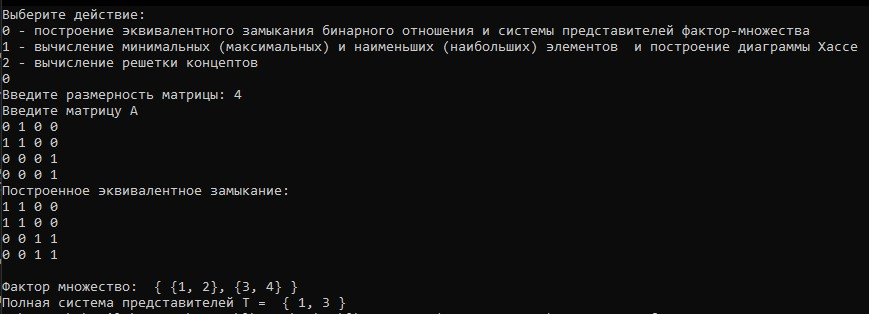
\includegraphics[width=0.9\textwidth]{test_1}
		\caption{Тестировние №1}
		\label{fig:test_1}
	\end{figure}
	
	Тестирование №2:
	
	Вычисление минимальных (максимальных) и наименьших (наибольших) элементов  и построение диаграммы Хассе. Ввод числом. Единица включается.
	
	\begin{figure}[H]
		\centering
		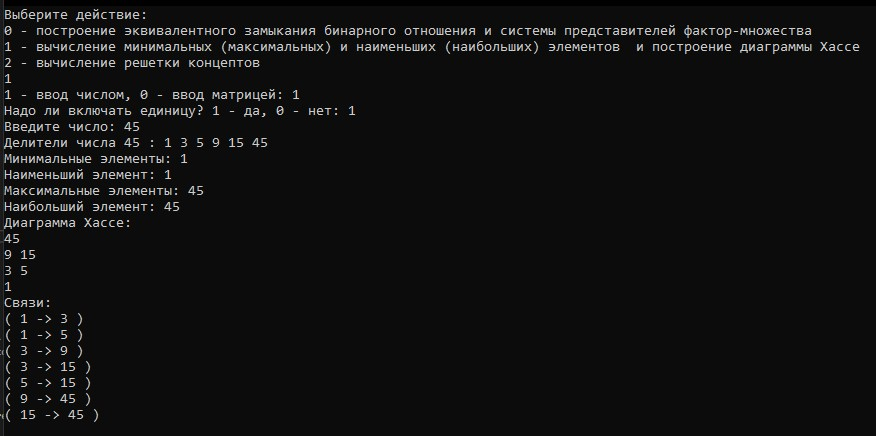
\includegraphics[width=0.9\textwidth]{test_2}
		\caption{Тестировние №2}
		\label{fig:test_2}
	\end{figure}
	
	Тестирование №3:

	Вычисление минимальных (максимальных) и наименьших (наибольших) элементов  и построение диаграммы Хассе. Ввод числом. Единица не включается.

	
	\begin{figure}[H]
		\centering
		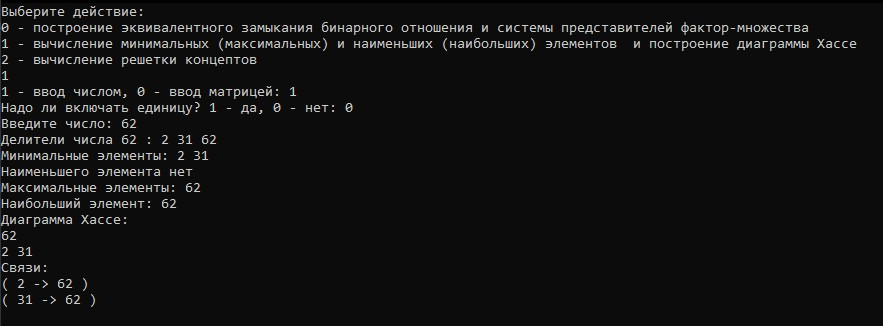
\includegraphics[width=0.9\textwidth]{test_3}
		\caption{Тестировние №3}
		\label{fig:test_3}
	\end{figure}

		Тестирование №4:
	
	Вычисление минимальных (максимальных) и наименьших (наибольших) элементов  и построение диаграммы Хассе. Ввод матрицей.
	
	
	\begin{figure}[H]
		\centering
		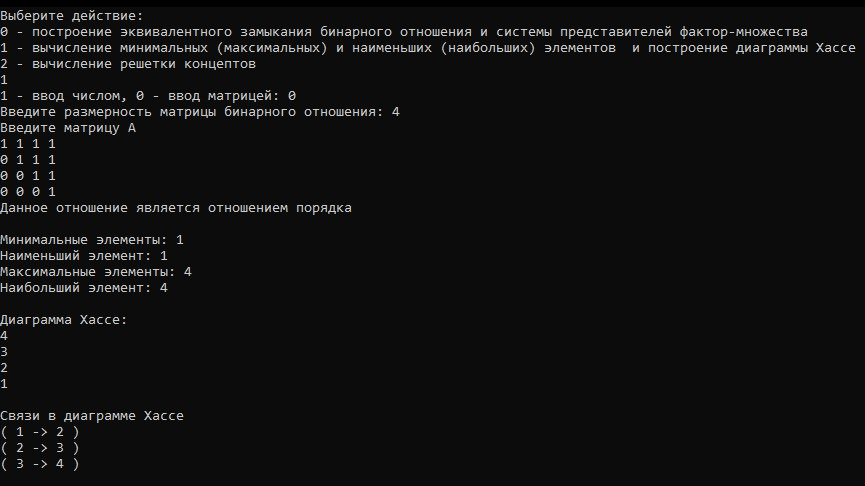
\includegraphics[width=0.9\textwidth]{test_4}
		\caption{Тестировние №4}
		\label{fig:test_4}
	\end{figure}
	
		Тестирование №5:
	
	Построение решетки концептов.
	
	
	\begin{figure}[H]
		\centering
		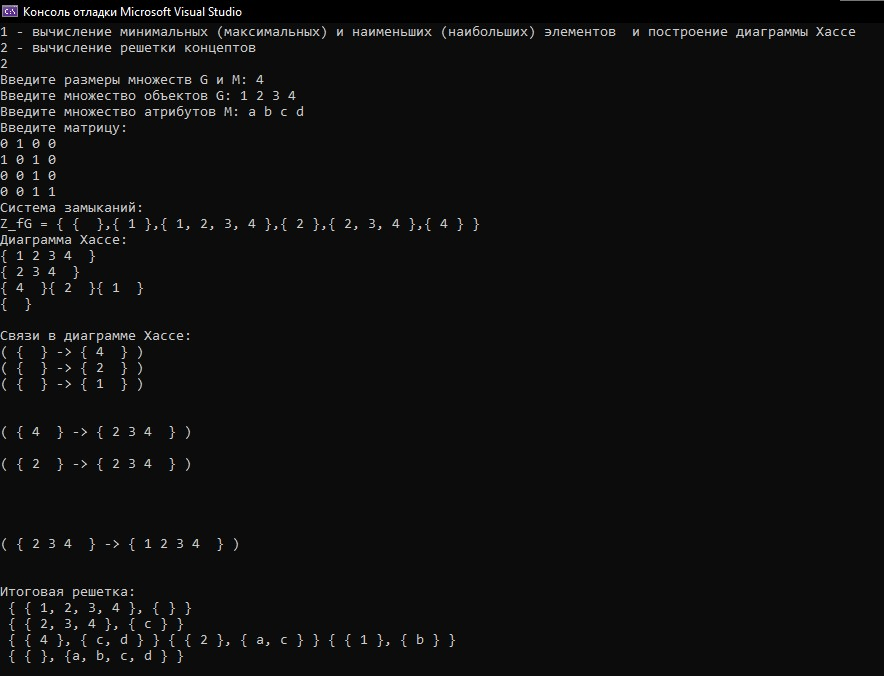
\includegraphics[width=0.9\textwidth]{test_5}
		\caption{Тестировние №5}
		\label{fig:test_5}
	\end{figure}
		
	\newpage
	\conclusion %заключение
	
	В данной лабораторной работе были рассмотрены и изучены следующие темы: определения отношения эквивалентности, фактор-множества, определения отношения порядка и диаграммы Хассе, определения контекста и концепта. В третьей части работы были реализованы алгоритмы построения эквивалентного замыкания бинарного отношения и системы представителей фактор-множества, алгоритмы вычисления минимальных (максимальных) и наименьших (наибольших) элементов  и построения диаграммы Хассе и алгоритм вычисления решетки концептов.
	
	
	
\end{document}